% !TEX encoding = IsoLatin2  % notwendige Zeile f"ur Mac-Benutzer (muss als Kommentar stehen); Windos-Benutzer k"onnen die Zeile l"oschen.

% LaTeX-Vorlage Version 3.0,  Juni 2010
% erstellt von Dr. Andreas Drauschke und Dr. Susanne Teschl
% Modifiziert von Dr. Andreas Mehrle (andreas.mehrle@mci.edu)

\documentclass[a4paper,oneside,10pt]{article}%{scrreprt} 
% F"ur kurze Arbeiten w"are auch die Dokumentklasse "scrartcl" ausreichend. In diesem Fall ist "section" die h"ochste Ebene ("chapter" gibt es dann nicht).
% \documentclass[a4paper,bibtotoc,oneside]{scrbook}

\usepackage{ifthen}
\newboolean{english}
%\setboolean{english}{true}		% auskommentieren fuer deutsche Version

\ifthenelse{\boolean{english}}
{}{
	\usepackage{german}
}
\usepackage[dvips]{graphicx}
\usepackage[tmargin=1in,bmargin=1in,lmargin=1.25in,rmargin=1.25in]{geometry}
\usepackage{titlesec}
\usepackage{xcolor}
\usepackage[overload]{textcase}
\definecolor{MSBlue}{rgb}{.204,.353,.541}
\definecolor{MSLightBlue}{rgb}{.31,.506,.741}
% Set formats for each heading level
%\titleformat*{\section}{\rmfamily\bfseries\huge\color{MSBlue}\lowercase}
\titleformat{\section}[hang]{\rmfamily\bfseries\huge\color{MSBlue}\lowercase}{\thesection}{1em}{}[]
\titleformat{\subsection}{\large\bfseries\sffamily\uppercase}{\thesubsection}{1em}{}
\titleformat{\subsubsection}{\sffamily\bfseries}{\thesubsubsection}{1em}{}
\renewcommand\contentsname{\ifthenelse{\boolean{english}}{table of contents.}{inhaltsverzeichnis.}}
\renewcommand\listfigurename{\ifthenelse{\boolean{english}}{list of figures.}{abbildungsverzeichnis.}}
\renewcommand\listtablename{\ifthenelse{\boolean{english}}{list of tables.}{tabellenverzeichnis.}}
\renewcommand\refname{\litname.}
\usepackage{exscale,relsize}
\usepackage{fancyhdr}
\usepackage[small]{caption}
\usepackage{float}
\usepackage{amsmath}
%\usepackage{units}
\usepackage{subfigure}
\usepackage{wallpaper}
\usepackage{pst-all}
\usepackage{amssymb}
\usepackage{rotating}
\usepackage[]{amsmath}
\usepackage{mathrsfs}
\usepackage{pgfplots}
\pgfplotsset{compat=1.18}
\usepackage{makeidx}
%\usepackage[pdftex,bookmarks=true,bookmarksnumbered=true]{hyperref}

\newcommand{\babel}[2]{\ifthenelse{\boolean{english}}{#1}{#2}}

% color set
\definecolorseries{foo}{rgb}{last}[rgb]{1.0,0.0,0.0}[rgb]{0.0,0.0,1.0}
\resetcolorseries[16]{foo}

% auxillary symbols
\renewcommand{\tilde}{\symbol{126}}
\newcommand{\define}{\stackrel{!}{=}}
\renewcommand{\equiv}{\,\widehat{=}\,}
\newcommand{\subsubsubsection}{\textbf}
\newcommand{\re}{\mathrm{Re}}
\newcommand{\pr}{\mathrm{Pr}}
\newcommand{\st}{\mathrm{St}}
\newcommand{\fr}{\mathrm{Fr}}
\newcommand{\nus}{\mathrm{Nu}}
\newcommand{\gr}{\mathrm{Gr}}
\newcommand{\ra}{\mathrm{Ra}}
\newcommand{\mif}{\quad\mathrm{\babel{if}{falls}}\quad}
\newcommand{\with}{\quad\mathrm{\babel{with}{mit}}\quad}
\newcommand{\for}{\quad\mathrm{\babel{for}{f"ur}}\quad}
%\renewcommand{\not}{\not}
\newcommand{\im}{i}
\newcommand{\ariwam}{ARiWaM}
\newcommand{\matlab}{MATLAB}

% format specifications
\renewcommand{\emph}{\textbf}
\newcommand{\file}{\textit}
\newcommand{\cmd}{\texttt}
\newcommand{\ten}{\boldsymbol}
%\newcommand{\unit}{\mathrm}
\newcommand{\lemma}{\textit}
\newcommand{\deutsch}[1]{german: \textit{#1}}
\renewcommand{\index}{\emph}

% Command path to graphic files
\newcommand{\gpath}{./grafics}
\newcommand{\bsppath}{../uebungen/beispiele}

% mathematical operators
\newcommand{\grad}{\,\mathrm{grad}\,}
\renewcommand{\div}{\,\mathrm{div}\,}
\newcommand{\rot}{\,\mathrm{rot}\,}
\newcommand{\lap}{\Delta}
\newcommand{\laplace}[1]{\mathscr{L}\left\{#1\right\}}
\newcommand{\trans}{^T}
\newcommand{\norm}{\psarc[linewidth=0.5pt](0,0){0.4}{0}{90}\psdot[dotsize=0.1](0.15,0.15)}

% electrical networks
\newcommand{\con}{\pscircle[linewidth=2pt,fillstyle=solid,fillcolor=black](0,0){0.1}}
\newcommand{\pin}{\pscircle[linewidth=2pt,fillstyle=solid](0,0){0.15}}
\newcommand{\link}{\psline[linewidth=2pt]}
\newcommand{\linkd}{\psline[linestyle=dashed]}
\newcommand{\arcd}{\psarc[linestyle=dashed]}
\newcommand{\arrow}{\psline[linewidth=2pt,arrowsize=8pt]{->}}
\newcommand{\cs}{\pscircle[linewidth=2pt](0,0){0.5}\arrow(0,-0.4)(0,0.4)\link(0,-0.5)(0,-2)\link(0,0.5)(0,2)}
\newcommand{\vs}{\pscircle[linewidth=2pt](0,0){0.5}\psline(-0.2,-0.1)(0.2,-0.1)\psline(-0.2,0)(0.2,0)\pscurve(-0.2,0.1)(-0.1,0.15)(0,0.1)(0.1,0.05)(0.2,0.1)\link(0,-0.5)(0,-2)\link(0,0.5)(0,2)}
\newcommand{\res}{\psframe[linewidth=2pt](-0.3,-1)(0.3,1)\link(0,-1)(0,-2)\link(0,1)(0,2)}
\newcommand{\ind}{\psframe[linewidth=2pt,fillstyle=solid,fillcolor=black](-0.3,-1)(0.3,1)\link(0,-1)(0,-2)\link(0,1)(0,2)}
\renewcommand{\cap}{\link(-0.5,-0.1)(0.5,-0.1)\link(-0.5,0.1)(0.5,0.1)\link(0,-0.1)(0,-2)\link(0,0.1)(0,2)}
\newcommand{\opv}{\pspolygon[linewidth=2pt](-1,-1.3)(-1,1.3)(1.3,0)\link(-1,-0.8)(-2,-0.8)\link(-1,0.8)(-2,0.8)\link(1.3,0)(2,0)\rput(-0.7,0.8){$-$}\rput(-0.7,-0.8){$+$}}

% mechanical networks
\newcommand{\mass}{\psframe[linewidth=2pt](-0.5,-0.5)(0.5,0.5)\link(0,0.5)(0,1)\link(0,-0.5)(0,-1)}
\newcommand{\spring}{\link(0,-1)(0,-0.8)(-0.3,-0.7)(0.3,-0.5)(-0.3,-0.3)(0.3,-0.1)(-0.3,0.1)(0.3,0.3)(-0.3,0.5)(0.3,0.7)(0,0.8)(0,1)}
\newcommand{\damp}{\link(-0.5,0.4)(-0.5,-0.3)(0.5,-0.3)(0.5,0.4)\link(-0.42,0.2)(0.42,0.2)\link(0,0.2)(0,1)\link(0,-0.3)(0,-1)}
\newcommand{\hatch}{\psframe[fillstyle=vlines,linestyle=none,hatchwidth=0.25pt]}
\newcommand{\clamp}{\hatch(-0.5,-0.3)(0.5,0)\link(-0.5,0)(0.5,0)}
\newcommand{\fixed}{\hatch(-0.5,-0.7)(0.5,-0.4)\link(-0.5,-0.4)(0.5,-0.4)\link(-0.25,-0.4)(0,0)(0.25,-0.4)\pscircle[linewidth=2pt,fillstyle=solid](0,0){0.1}}
\newcommand{\loose}{\hatch(-0.5,-0.7)(0.5,-0.5)\link(-0.5,-0.4)(0.5,-0.4)\link(-0.5,-0.5)(0.5,-0.5)\link(-0.25,-0.4)(0,0)(0.25,-0.4)\pscircle[linewidth=2pt,fillstyle=solid](0,0){0.1}}
\newcommand{\axial}{\link(-0.3,-0.3)(-0.3,-0.1)(0.3,-0.1)(0.3,-0.3)\link(-0.3,0.3)(-0.3,0.1)(0.3,0.1)(0.3,0.3)}
\newcommand{\force}{\psline[linewidth=2pt,arrowsize=6pt]{->}}
\newcommand{\rmom}{\psarc[arrowsize=6pt,linewidth=2pt]{<-}}
\newcommand{\lmom}{\psarc[arrowsize=6pt,linewidth=2pt]{->}}
\newcommand{\stress}{\psline[arrowsize=6pt]{->}}
\newcommand{\beam}{\psframe[fillstyle=solid,fillcolor=lightgray]}
\newcommand{\rod}{\psline[linewidth=3pt]}
\newcommand{\disp}{\psline[linewidth=2pt,arrowsize=6pt]{->}}	% displacement

% hydraulical networks
\newcommand{\pump}{\pscircle[linewidth=2pt,fillstyle=solid,fillcolor=white](0,0){1}\pspolygon[fillstyle=solid,fillcolor=black](0,1)(-0.15,0.3)(0.15,0.3)}
\newcommand{\motor}{\pscircle[linewidth=2pt,fillstyle=solid,fillcolor=white](0,0){0.8}\rput(0,0){M}}
\newcommand{\throttle}{\psarc[linewidth=2pt](-3,0){2.7}{-15}{15}\psarc[linewidth=2pt](3,0){2.7}{165}{195}}
\newcommand{\limiter}{\psframe[linewidth=2pt,fillstyle=solid,fillcolor=white](-0.7,-0.7)(0.7,0.7)\psline{->}(-0.5,-0.4)(-0.5,0.1)(0.5,-0.25)}

% diagrams (block and s-plane)
\newcommand{\axis}{\psline[arrowsize=6pt,arrowinset=0]{->}}
\newcommand{\measure}{\psline[linewidth=0.5pt,arrowsize=4pt]}
\newcommand{\xtick}[1]{\measure(#1,-0.1)(#1,0.1)}
\newcommand{\ytick}[1]{\measure(-0.1,#1)(0.1,#1)}
\newcommand{\psang}{\psarc[linewidth=0.5pt,arrowsize=4pt]{<->}}
\newcommand{\tf}[1]{\psframe[linewidth=2pt](-1,-0.75)(1,0.75)\rput(0,0){#1}}
\newcommand{\tff}[2]{\psframe[fillstyle=solid,fillcolor=lightgray](-1,0)(1,0.75)\psframe[linewidth=2pt](-1,-0.75)(1,0.75)\rput(0,0.35){#1}\rput(0,-0.35){#2}}
\newcommand{\sat}{\psframe[linewidth=2pt](-1,-0.75)(1,0.75)\link(-0.8,-0.5)(-0.5,-0.5)(0.5,0.5)(0.8,0.5)}
\newcommand{\add}[4]{\pscircle[linewidth=2pt,fillstyle=solid,fillcolor=white](0,0){0.5}\rput(-0.5,-0.75){#1}\rput(-0.75,0.5){#2}\rput(0.5,0.75){#3}\rput(0.75,-0.5){#4}}
\newcommand{\pole}{\link(-0.15,-0.15)(0.15,0.15)\link(-0.15,0.15)(0.15,-0.15)}
\newcommand{\zero}{\pscircle[linewidth=2pt,fillstyle=solid](0,0){0.15}}
\newcommand{\textblock}[1]{\psframebox[linewidth=2pt]{\parbox[c][2cm][c]{3cm}{\centering #1}}}

% thermodynamic systems
\newcommand{\cv}{\psframe[linestyle=dashed]}
\newcommand{\sys}{\psframe[fillcolor=white,fillstyle=solid,linewidth=2pt]}
\newcommand{\iso}{\psframe[linewidth=2pt,fillstyle=vlines]}
\newcommand{\candle}{\psframe[linewidth=0.5pt](-0.15,-0.5)(0.15,0.3)\pscurve[linewidth=0.5pt](0,0.8)(-0.1,0.5)(0,0.3)(0.1,0.5)(0,0.8)\pscurve[linewidth=0.5pt](0,0.6)(-0.08,0.4)(0,0.3)(0.08,0.4)(0,0.6)}
\newcommand{\flux}{\psline[arrowsize=10pt,linewidth=4pt]{->}}
\newcommand{\point}[1]{\pscircle(0,0){0.3}\rput[c](0,0){#1}}

% aerodynamics
\newcommand{\source}{\pin\rput{0}(0,0){\arrow(0.5,0)(1,0)}\rput{45}(0,0){\arrow(0.5,0)(1,0)}\rput{90}(0,0){\arrow(0.5,0)(1,0)}\rput{135}(0,0){\arrow(0.5,0)(1,0)}\rput{180}(0,0){\arrow(0.5,0)(1,0)}\rput{225}(0,0){\arrow(0.5,0)(1,0)}\rput{270}(0,0){\arrow(0.5,0)(1,0)}\rput{315}(0,0){\arrow(0.5,0)(1,0)}}

% CFD
\newcommand{\cell}[1]{\definecolor{cellc}{gray}{#1}\psframe[linewidth=2pt,fillstyle=solid,fillcolor=cellc](0,0)(1,1)}

%\renewcommand{\labelenumi}{\alph{enumi})}

\setlength{\parindent}{0em}
\setlength{\parskip}{1.5ex plus0.5ex minus0.5ex}
\setlength{\captionmargin}{3em}

% counters
\newcounter{example}
\ifthenelse{\boolean{english}}{\newcommand{\exampletext}{example }}{\newcommand{\exampletext}{Beispiel }}
\newcommand{\example}[1]{\underline{\exampletext \arabic{chapter}.\arabic{example}:} #1 \addtocounter{example}{1}}
\newcounter{exercise}
\ifthenelse{\boolean{english}}{\newcommand{\exercisetext}{exercise }}{\newcommand{\exercisetext}{Aufgabe }}
\newcommand{\exercise}[1]{\underline{\exercisetext \arabic{chapter}.\arabic{exercise}:} #1 \stepcounter{exercise}}
\newcommand{\cchapter}[1]{\chapter{#1} \setcounter{example}{1} \setcounter{exercise}{1}}
\ifthenelse{\boolean{english}}{\newcommand{\solution}{\textit{solution:} }}{\newcommand{\solution}{\textit{L\"osung:} }}
%\newcounter{beispiel}
%\setcounter{beispiel}{1}		% Nummer des ersten Beispiels
\newboolean{student}
\newcounter{enumcount}
\newcommand{\resume}[1]{\begin{#1} \setcounter{enumi}{\value{enumcount}}}
\newcommand{\pause}[1]{\setcounter{enumcount}{\value{enumi}} \end{#1}}




\def\labtitle{Biosignalverarbeitung Labor}
\def\labcode{MGST-B-3-BB-BS-ILV}
\def\labname{Aufbau der Hardware \& Datenakquise}
\def\labnum{1}

\def\study{Bachelor Medizin,- Gesundheits- und Sporttechnologie}
\def\term{3.}
\def\lecturer{Gerda Strutzenberger, Aitor Morillo Rascon}
\def\group{MGST 2025}
\def\student{Johanna Helfer, Nele Janina Hinz , Luisa Kneppel}

\def\litname{literatur}

\begin{document}

%\layout

% Kopf- und Fusszeilen initiieren
\pagestyle{plain}

% Deckblatt:
\thispagestyle{empty}
\sffamily
%\put(-30,-685){\includegraphics[width=1.15\linewidth]{BG}}

{\bfseries


\vspace*{1cm}

\def\thesis{\ifthenelse{\boolean{english}}{laboratory report}{laborbericht}}
\textcolor{MSBlue}{\rmfamily\bfseries\huge\thesis.}%

\vspace*{0.5cm}

\textbf{\labtitle{ }(\labcode)}

\labname

\ifthenelse{\boolean{english}}{Lab}{Labor} \labnum

\vspace*{10cm}

\textcolor{gray}{\study}

\def\termname{\ifthenelse{\boolean{english}}{semester}{Semester}}
\textcolor{gray}{\term{ }\termname}

\def\lecturername{\ifthenelse{\boolean{english}}{Responsible lecturer}{Lehrveranstaltungsleiter}}
\textcolor{gray}{\lecturername: \lecturer}

\def\groupname{\ifthenelse{\boolean{english}}{Group}{Jahrgang}}
\textcolor{gray}{\groupname: \group}

\def\authorname{\ifthenelse{\boolean{english}}{Author}{Verfasser}}
\textcolor{gray}{\authorname: \student}

\textcolor{gray}{\today}

\newpage}


\tableofcontents%\thispagestyle{empty}
\listoffigures
\listoftables

\newpage

% Kopf- und Fusszeilen initiieren
\pagestyle{fancy}

\section{Einleitung}
Ziel des Laborversuchs ist es, die Grundlagen der Datenerfassung und Signalverarbeitung anhand eines 
Beschleunigungssensors kennenzulernen.
Hierfür werden statische und dynamische Messungen durgeführt, die Sensoreinstellungen verändert 
und die Auswirkungen auf die Messdaten untersucht.
\newline
Die aufgenommenen Daten werden mit Python ausgewertet und grafisch dargestellt.

\section{Grundlagen und Messsystem}
\subsection{Aufbau und Funktionsweise des Messsystems}
HIER GRAFIK UND BESCHREIBUNG!!
\subsection{Temperaturmessung mithilfe eines Sensors}
Die Körpertemperatur wird mithilfe eines Sensors bestimmt, der Spannungen von
$0$ bis $3{,}3\,\mathrm{V}$ messen kann und einen Messbereich von 
$0$ bis $40\,^\circ\mathrm{C}$ hat. Der Microcontroller, der die Sensordaten
verbeitet und digitalisiert, kann bis zu $5\,\mathrm{V}$ und und mit einer Auflösung 
von $10\,\mathrm{Bit}$ messen.
Für einen ausgegebenen Messwert von $520$
soll die entsprechende Temperatur berechnet werden.
\newline
\newline
\textbf{1. Berechnung der Sensorspannung aus dem ADC-Messwert}

Ein 10-Bit-ADC kann $2^{10}=1024$ unterschiedliche Werte darstellen.
Der digitale Wertebereich reicht also von $0$ bis $1023$.

Die Auflösung (kleinstmögliche messbare Spannungsänderung in Volt) lässt sich
aus folgender Formel berechnen (siehe Vorlesungsfolien, S. 14)\cite{vorlesung_signalerfassung}:

\begin{equation}
    \Delta V = \frac{V_{\mathrm{FS}}}{2^N}
\end{equation}

Dabei bezeichnet $V_{\mathrm{FS}}$ den Messbereich des ADC (Full Scale)
und $N$ die Bit-Tiefe.

Durch Einsetzen der gegebenen Werte ergibt sich:

\begin{equation}
    \Delta V = \frac{5\,\mathrm{V}}{2^{10}}
    = 0{,}004883\,\mathrm{V}
\end{equation}
\newline
Die Sensorauflösung beträgt somit ungefähr $4{,}88\,\mathrm{mV}$.
\newline
Im nächsten Schritt wird die Sensorspannung durch folgende Formel berechnet:

\begin{equation}
    U_{\mathrm{Sensor}} =
    ADC_{\mathrm{Wert}} \cdot \Delta V
\end{equation}

Mit dem gegebenen Messwert von $520$ ergibt sich:

\begin{equation}
    U_{\mathrm{Sensor}} =
    520 \cdot 0{,}004883\,\mathrm{V}
\end{equation}

\begin{equation}
    \boxed{U_{\mathrm{Sensor}} \approx 2{,}539\,\mathrm{V}}
\end{equation}

\textbf{2. Umrechnung der Spannung in eine Temperatur}

Aus der Aufgabenstellung geht hervor, dass ein linearer Zusammenhang
zwischen der Sensorspannung und der Temperatur besteht.

\begin{equation}
    \frac{U_{\mathrm{Sensor}}}{U_{\mathrm{Sensor,max}}}
    =
    \frac{T}{T_{\mathrm{max}}}
\end{equation}

Durch Umstellen der Gleichung nach $T$ ergibt sich:
\begin{equation}
    T =
    \frac{U_{\mathrm{Sensor}}}{U_{\mathrm{Sensor,max}}}
    \cdot T_{\mathrm{max}}
\end{equation}

Werden die gegebenen Werte und die zuvor berechnete Spannung 
in die Gleichung eingesetzt, ergibt sich:

\begin{equation}
    T =
    \frac{2{,}539\,\mathrm{V}}{3{,}3\,\mathrm{V}}
    \cdot 40\,^\circ\mathrm{C}
\end{equation}

Daraus folgt:

\begin{equation}
    \boxed{T \approx 30{,}8\,^\circ\mathrm{C}}
\end{equation}

Der ADC-Messwert von $520$ entspricht somit einer Temperatur
von ungefähr $30{,}8\,^\circ\mathrm{C}$.

\subsection{Beschleunigungssensor: Koordinatensystem und Skalierung}

Der im Versuch verwendete Beschleunigungssensor MMA8452Q
von NXP misst die Beschleunigung entlang drei orthogonaler
Raumachsen (X, Y und Z). Dadurch können Beschleunigungen
in allen drei Raumrichtungen erfasst werden.

\textbf{Achsenzuordnung und Überprüfung}

Zur Überprüfung der Achsenzuordnung wurde der Sensor
unterschiedlich ausgerichtet. Dazu wurde er zunächst
auf eine ebene Fläche gelegt und anschließend so gedreht,
dass jeweils eine der drei Achsen senkrecht nach oben
bzw. unten zeigte.

Aufgrund der Erdbeschleunigung sollte bei einer ruhenden
und entsprechend ausgerichteten Sensorachse ein Wert
von ungefähr $+1\,g$ oder $-1\,g$ gemessen werden.
Die beiden anderen Achsen sollten dabei jeweils
annähernd $0\,g$ anzeigen. Das Vorzeichen hängt von
der Orientierung des Sensors und der jeweiligen
Achsenkonvention ab.

Durch diesen Versuch lässt sich feststellen, welcher
der drei ausgegebenen Messwerte der jeweiligen
Sensorachse zugeordnet ist.
Zur Überprüfung der Achsenzuordnung wurde der Sensor
unterschiedlich ausgerichtet. Dazu wurde er zunächst
auf eine ebene Fläche gelegt und anschließend so gedreht,
dass jeweils eine der drei Achsen senkrecht nach oben
bzw. unten zeigte.

\begin{figure}[H]
    \centering
    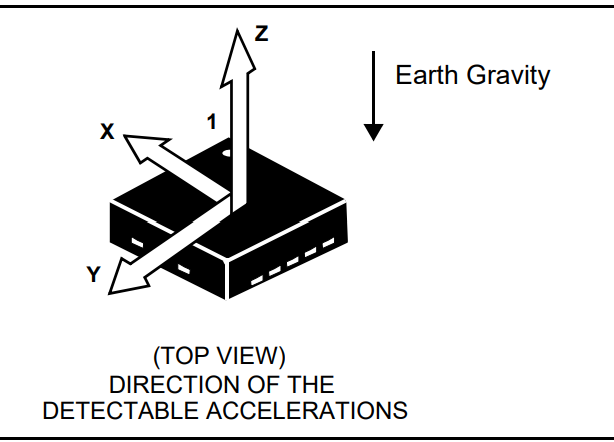
\includegraphics[width=0.65\textwidth]{Abbildungen/Achsen.png}
    \caption{Koordinatensystem und Achsen des Beschleunigungssensors MMA8452Q. Quelle: NXP, Datenblatt MMA8452Q, S. 3 \cite{nxp_mma8452q}.}
    \label{fig:mma8452q}
\end{figure}

Aufgrund der Erdbeschleunigung sollte bei einer ruhenden
und entsprechend ausgerichteten Sensorachse ein Wert
von ungefähr $+1\,g$ oder $-1\,g$ gemessen werden.

\textbf{Einheit und Empfindlichkeit der Messwerte}

Der MMA8452Q besitzt eine digitale Auflösung von
12 Bit. Die Beschleunigungswerte werden zunächst als
vorzeichenbehaftete digitale Rohwerte (Counts)
ausgegeben. Diese stellen noch keine physikalischen
Beschleunigungswerte in $\mathrm{m/s^2}$ dar.

Die Empfindlichkeit hängt vom eingestellten
Messbereich ab. Laut Datenblatt des Herstellers
NXP ergeben sich folgende Werte:

\begin{itemize}
    \item Messbereich $\pm 2\,g$: 1024 Counts/g
    \item Messbereich $\pm 4\,g$: 512 Counts/g
    \item Messbereich $\pm 8\,g$: 256 Counts/g
\end{itemize}

Diese Angaben sind im Datenblatt des MMA8452Q
in Abschnitt 3.1 auf Seite 10 beschrieben
\cite{MMA8452Q}.

\textbf{Umrechnung in die physikalische Einheit
$\mathrm{m/s^2}$}

Die Umrechnung der digitalen Rohwerte in eine
physikalische Beschleunigung erfolgt in zwei Schritten.
Zunächst werden die Counts anhand der jeweiligen
Empfindlichkeit in die Einheit $g$ umgerechnet.
Anschließend erfolgt die Umrechnung in
$\mathrm{m/s^2}$ durch Multiplikation mit der
Erdbeschleunigung von $9{,}80665\,\mathrm{m/s^2}$.

Allgemein gilt:

\begin{equation}
    a_g = \frac{\text{Rohwert}}{\text{Empfindlichkeit}}
\end{equation}

Die Umrechnung in die physikalische Einheit ergibt:

\begin{equation}
    a = a_g \cdot 9{,}80665\,\mathrm{m/s^2}
\end{equation}

Für den im ersten Arduino-Code verwendeten Messbereich
von $\pm 2\,g$ erfolgt die Einstellung über:

\begin{center}
    \texttt{accel.setScale(SCALE\_2G);}
\end{center}

Mit einer Empfindlichkeit von 1024 Counts/g ergibt
sich somit:

\begin{equation}
    \boxed{
    a = \frac{\text{Rohwert}}{1024}
    \cdot 9{,}80665\,\mathrm{m/s^2}
    }
\end{equation}

Für den Messbereich von $\pm 8\,g$, welcher im
zweiten Arduino-Code verwendet wird, gilt:

\begin{center}
    \texttt{accel.setScale(SCALE\_8G);}
\end{center}

Da die Empfindlichkeit hier 256 Counts/g beträgt,
lautet die entsprechende Umrechnungsformel:

\begin{equation}
    \boxed{
    a = \frac{\text{Rohwert}}{256}
    \cdot 9{,}80665\,\mathrm{m/s^2}
    }
\end{equation}

\textbf{Bedeutung des Messbereichs}

Die Wahl des Messbereichs beeinflusst sowohl die
maximal erfassbare Beschleunigung als auch die
Auflösung der Messung. Ein kleinerer Messbereich
ermöglicht eine höhere Empfindlichkeit, während
ein größerer Messbereich höhere Beschleunigungen
erfassen kann.

Wird der eingestellte Messbereich überschritten,
erreicht der Sensor seine Messgrenze. Dieses
Verhalten wird als Sättigung bezeichnet. Die
gemessenen Beschleunigungswerte können dann nicht
mehr vollständig dargestellt werden.

\section{Dynamische Beschleunigungsmessung}

\subsection{Durchführung und Darstellung der Messung (Aufgabe 4a)}

Für die dynamische Beschleunigungsmessung wurde der Beschleunigungssensor gemäß der Versuchsanleitung mit dem Arduino-Code \texttt{Lab1Code1} betrieben. Der Sensor wurde in der geschlossenen Hand gehalten und für etwa zehn Sekunden möglichst gleichmäßig einmal pro Sekunde auf und ab bewegt. Die vom Sensor erfassten Messwerte wurden über den seriellen Monitor ausgegeben und anschließend zur weiteren Verarbeitung in einer Textdatei gespeichert.

Für die Auswertung wurden vier Sekunden der aufgezeichneten Messdaten ausgewählt und grafisch dargestellt. Dabei wurde die Beschleunigung über der Zeit aufgetragen.

% HIER DEN PLOT EINFÜGEN
% Beispiel:
% \begin{figure}[H]
%     \centering
%     \includegraphics[width=0.85\textwidth]{Abbildungen/Aufgabe4a.png}
%     \caption{Beschleunigungssignal während der dynamischen Auf- und Abbewegung des Sensors.}
%     \label{fig:aufgabe4a}
% \end{figure}

\subsection{Plateaus der Signalpeaks (Aufgabe 4b)}

In den aufgezeichneten Beschleunigungssignalen können an den Spitzen der Peaks Plateaus auftreten. Diese entstehen durch eine Sättigung des Beschleunigungssensors. Bei der verwendeten Einstellung \texttt{SCALE\_2G} beträgt der Messbereich des Sensors ungefähr $-2g$ bis $+2g$. Überschreitet die tatsächliche Beschleunigung diesen Bereich, kann der Sensor den Wert nicht mehr korrekt erfassen. Stattdessen wird der maximal darstellbare Messwert ausgegeben. Dadurch werden die Spitzen des Signals abgeschnitten und es entstehen Plateaus. Die Plateaus liegen jeweils auf demselben Wert, da der Sensor bei Überschreiten seines Messbereichs immer denselben maximalen beziehungsweise minimalen digitalen Wert ausgibt.

Eine Möglichkeit, dieses Problem zu reduzieren, besteht darin, den Messbereich des Sensors zu vergrößern. Der MMA8452Q bietet hierfür die Einstellungen $\pm 2g$, $\pm 4g$ und $\pm 8g$. Bei einem größeren Messbereich können höhere Beschleunigungen erfasst werden, allerdings nimmt gleichzeitig die Empfindlichkeit ab. Bei einer Auflösung von 12 Bit ergeben sich folgende Empfindlichkeiten:

\begin{itemize}
    \item $\pm 2g$: 1024 Counts/g
    \item $\pm 4g$: 512 Counts/g
    \item $\pm 8g$: 256 Counts/g
\end{itemize}

Die Wahl des Messbereichs hängt somit von der jeweiligen Anwendung ab. Für geringe Beschleunigungen ist ein kleiner Messbereich vorteilhaft, während für stärkere Bewegungen ein größerer Messbereich gewählt werden sollte.

\subsection{Abweichungen zwischen Bewegung und Messsignal (Aufgabe 4c)}

Die aufgezeichneten Messdaten stellen die tatsächlich ausgeführte Handbewegung nicht exakt dar, da der Beschleunigungssensor nicht die Position oder Geschwindigkeit, sondern die Beschleunigung misst. Daher entspricht der Verlauf des Messsignals nicht unmittelbar der sichtbaren Bewegung des Sensors. Zusätzlich überlagert die Erdbeschleunigung das gemessene Signal. Auch die Handbewegung selbst erfolgt nicht vollkommen gleichmäßig oder sinusförmig, wodurch Schwankungen im Signal entstehen können.

Ein weiterer Einflussfaktor ist die Abtastrate des Sensors, die durch die sogenannte Output Data Rate (ODR) festgelegt wird. Sie gibt an, wie viele neue Messwerte pro Sekunde bereitgestellt werden. Bei einer zu niedrigen Abtastrate können schnelle Änderungen der Beschleunigung nicht ausreichend erfasst werden. Während des Versuchs wurde die Abtastrate daher angepasst. Bei einer Einstellung von 1 Hz werden lediglich ein Messwert pro Sekunde erfasst, während bei 200 Hz deutlich mehr Messwerte zur Verfügung stehen. Dadurch kann der zeitliche Verlauf der Bewegung genauer dargestellt werden. Weitere Abweichungen können durch Messrauschen, interne Filterung des Sensors und eine mögliche Sättigung bei Überschreiten des eingestellten Messbereichs entstehen.


\section{Anpassung der Abtastrate und Vergleich der Messungen}

\subsection{Konfiguration des Beschleunigungssensors (Aufgabe 5)}

Um die aufgezeichneten Messdaten besser an die tatsächlich ausgeführte Bewegung anzupassen, wurde die Konfiguration des Beschleunigungssensors MMA8452Q anhand des Datenblatts untersucht und der Arduino-Code entsprechend angepasst.

Der Messbereich des Sensors wird über das Register \texttt{XYZ\_DATA\_CFG} (Adresse 0x0E) eingestellt. Die entsprechenden Einstellungen sind in Abschnitt 6.1 des Datenblatts in Tabelle 15 und Tabelle 16 beschrieben. Die Bits FS[1:0] legen den Full-Scale-Bereich fest. Dabei entsprechen die Bitkombinationen 00, 01 und 10 den Messbereichen $\pm 2g$, $\pm 4g$ und $\pm 8g$. Die Kombination 11 ist reserviert.

Die Empfindlichkeit des Sensors hängt vom gewählten Messbereich ab. Laut Tabelle 2 des Datenblatts (S. 6) beträgt sie bei $\pm 2g$ 1024 Counts/g, bei $\pm 4g$ 512 Counts/g und bei $\pm 8g$ 256 Counts/g. Ein größerer Messbereich ermöglicht somit die Erfassung höherer Beschleunigungen, reduziert jedoch die Auflösung. Deshalb sollte der Messbereich möglichst klein gewählt werden, solange keine Sättigung auftritt.

Für die zeitliche Erfassung der Bewegung ist außerdem die Output Data Rate (ODR) entscheidend. Diese wird über die Bits DR[2:0] des Registers \texttt{CTRL\_REG1} (Adresse 0x2A) eingestellt. Die möglichen Einstellungen sind in Abschnitt 6.7, Tabelle 53 und Tabelle 55 des Datenblatts (S. 40) aufgeführt. Der Sensor unterstützt dabei Abtastraten von 1,56 Hz, 6,25 Hz, 12,5 Hz, 50 Hz, 100 Hz, 200 Hz, 400 Hz und 800 Hz.

Für die erneute Messung wurde eine Abtastrate von 200 Hz gewählt. Dies entspricht der Bitkombination 010 der Bits DR[2:0] und einer Abtastperiode von 5 ms. Durch die höhere Abtastrate stehen mehr Messpunkte pro Zeiteinheit zur Verfügung, wodurch schnelle Änderungen der Beschleunigung genauer erfasst werden können.

\subsection{Vergleich der Messungen}

Nach der Anpassung der Sensorkonfiguration wurde das Experiment erneut durchgeführt. Dabei wurde der Sensor wieder für etwa zehn Sekunden in der geschlossenen Hand einmal pro Sekunde auf und ab bewegt. Anschließend wurden erneut vier Sekunden der Messdaten ausgewählt und grafisch dargestellt.

% HIER DEN NEUEN PLOT EINFÜGEN
% Beispiel:
% \begin{figure}[H]
%     \centering
%     \includegraphics[width=0.85\textwidth]{Abbildungen/Aufgabe5.png}
%     \caption{Beschleunigungssignal nach Anpassung der Sensorkonfiguration mit einer ODR von 200 Hz.}
%     \label{fig:aufgabe5}
% \end{figure}

Im Vergleich zur vorherigen Messung ist durch die höhere Abtastrate eine genauere zeitliche Darstellung der Beschleunigungsänderungen zu erwarten. Der Signalverlauf kann dadurch der ausgeführten Handbewegung besser folgen. Gemeinsamkeiten zwischen beiden Messungen ergeben sich durch die gleiche Bewegungsdurchführung und die weiterhin vorhandene Erdbeschleunigung. Unterschiede können insbesondere durch die höhere Anzahl an Messpunkten und die dadurch verbesserte zeitliche Auflösung entstehen. Eine mögliche Sättigung der Signalpeaks wird durch die Erhöhung der Abtastrate allein jedoch nicht behoben, da diese vom eingestellten Messbereich des Sensors abhängt.

\section{Statische Beschleunigungsmessung und Signalfilterung}

\subsection{Messung der sechs Sensororientierungen (Aufgabe 6)}

Zur Überprüfung der Beschleunigungsmessung wurden alle drei Achsen des MMA8452Q jeweils nach oben und nach unten ausgerichtet. Daraus ergeben sich insgesamt sechs verschiedene Sensororientierungen. Für jede Orientierung wurde eine Messdauer von etwa zehn Sekunden verwendet.

Bei ruhendem Sensor sollte jeweils die vertikale Achse eine Beschleunigung von ungefähr $1g$ beziehungsweise $-1g$ anzeigen. Die beiden horizontal ausgerichteten Achsen sollten dagegen Werte nahe $0g$ liefern. Das Vorzeichen hängt von der jeweiligen Orientierung und der Achsendefinition des Sensors ab.

Die aufgezeichneten Messwerte wurden gemeinsam in einem Diagramm dargestellt.

% HIER PLOT MIT ALLEN SECHS ORIENTIERUNGEN EINFÜGEN
% \begin{figure}[H]
%     \centering
%     \includegraphics[width=0.9\textwidth]{Abbildungen/Aufgabe6.png}
%     \caption{Beschleunigungsmessungen für die sechs verschiedenen Sensororientierungen.}
%     \label{fig:aufgabe6}
% \end{figure}

Anhand der Messwerte wird überprüft, ob die erwarteten Beschleunigungswerte von ungefähr $\pm 1g$ auf der jeweils vertikalen Achse erreicht werden. Abweichungen können beispielsweise durch eine ungenaue Ausrichtung des Sensors, Messrauschen oder Offsetfehler entstehen.

\subsection{Vergleich gefilterter und ungefilterter Messdaten (Aufgabe 7)}

Zur Untersuchung der Signalfilterung wurden die ursprünglichen Messdaten mit den gefilterten Messdaten verglichen. Hierfür wurde ein Tiefpassfilter in Form eines gleitenden Mittelwerts verwendet.

% HIER PLOT MIT GEFILTERTEN UND UNGEFILTERTEN DATEN EINFÜGEN
% \begin{figure}[H]
%     \centering
%     \includegraphics[width=0.9\textwidth]{Abbildungen/Aufgabe7.png}
%     \caption{Vergleich der ungefilterten und gefilterten Beschleunigungsdaten.}
%     \label{fig:aufgabe7}
% \end{figure}

Der Tiefpassfilter reduziert hochfrequentes Messrauschen und glättet dadurch den Signalverlauf. Da die eigentliche Handbewegung deutlich langsamer als das hochfrequente Rauschen ist, verbessert die Filterung die Darstellung des Nutzsignals. Allerdings können dadurch schnelle Signaländerungen abgeschwächt und die Peaks leicht verzögert beziehungsweise abgeflacht werden.

\subsection{Bestimmung der Abtastfrequenz (Aufgabe 8)}

Zur Bestimmung der tatsächlichen Abtastfrequenz wurde jedem Messwert während der Datenerfassung ein Zeitstempel direkt auf dem Mikrocontroller zugeordnet. Hierfür wurde eine Zeitfunktion des Mikrocontrollers verwendet. Die Zeitstempel wurden gemeinsam mit den Beschleunigungswerten gespeichert.

Aus den Zeitstempeln wurden zunächst die zeitlichen Abstände zwischen zwei aufeinanderfolgenden Messungen berechnet:

\begin{equation}
    \Delta t_i = t_{i+1} - t_i
\end{equation}

Die mittlere Abtastfrequenz ergibt sich aus dem Kehrwert des mittleren zeitlichen Abstands:

\begin{equation}
    f_s = \frac{1}{\overline{\Delta t}}
\end{equation}

Die Standardabweichung der zeitlichen Abstände beschreibt die Schwankung der Messintervalle:

\begin{equation}
    \sigma_{\Delta t} =
    \sqrt{
    \frac{1}{N-1}
    \sum_{i=1}^{N}
    (\Delta t_i-\overline{\Delta t})^2
    }
\end{equation}

% HIER PLOT DER ZEITABSTÄNDE ODER HISTOGRAMM EINFÜGEN
% \begin{figure}[H]
%     \centering
%     \includegraphics[width=0.85\textwidth]{Abbildungen/Aufgabe8.png}
%     \caption{Verteilung der zeitlichen Abstände zwischen aufeinanderfolgenden Messungen.}
%     \label{fig:aufgabe8}
% \end{figure}

Die berechnete mittlere Abtastfrequenz beträgt [WERT] Hz. Die Standardabweichung der zeitlichen Abstände beträgt [WERT] ms. Damit lässt sich beurteilen, wie konstant die Messintervalle während der Datenerfassung waren.

\subsection{Vergleich mit dem mobilen Messsystem (Aufgabe 9)}

Im letzten Versuchsteil wurde das mobile Messsystem mit DataLogger und Batterie verwendet. Die Datenerfassung erfolgte mit dem Arduino-Code \texttt{Lab1Code2} über einen Zeitraum von ungefähr zehn Sekunden.

Die Abtastfrequenz wurde erneut anhand der gespeicherten Zeitstempel bestimmt. Anschließend wurden die Ergebnisse mit der zuvor gemessenen Abtastfrequenz des ersten Messsystems verglichen.

Die mittlere Abtastfrequenz des mobilen Messsystems beträgt [WERT] Hz. Die zugehörige Standardabweichung beträgt [WERT] ms.

Unterschiede zwischen den beiden Messsystemen können durch die unterschiedlichen Abläufe der Datenerfassung entstehen. Insbesondere Schreibzugriffe auf die SD-Karte benötigen unterschiedlich lange und können dadurch Schwankungen der Messintervalle verursachen. Auch die unterschiedliche Programmstruktur sowie die serielle Datenübertragung des ersten Messsystems können die Abtastfrequenz beeinflussen.

\bibliographystyle{IEEEtran}	
\bibliography{Literatur}

\end{document}
